\documentclass[border=3pt]{standalone}
% Shared preamble for every generated figure.
% Matches the report: newtx (Times), greyscale, square boxes.
\usepackage{newtxtext,newtxmath}
% newtx's typewriter (txtt) draws a slashed zero; use Latin Modern instead.
\renewcommand{\ttdefault}{lmtt}
\usepackage{tikz}
\usetikzlibrary{positioning,arrows.meta,calc,fit,backgrounds,shapes.geometric,
                decorations.pathreplacing,decorations.pathmorphing,matrix,patterns}

\definecolor{figgrey}{gray}{0.88}
\definecolor{figmid}{gray}{0.60}
\definecolor{figdark}{gray}{0.35}

\tikzset{
  fig/.style={font=\small},
  box/.style={draw,thick,minimum height=8mm,minimum width=22mm,align=center,
              inner sep=2pt,font=\small},
  greybox/.style={box,fill=figgrey},
  smallbox/.style={draw,minimum height=6mm,minimum width=16mm,align=center,
                   inner sep=2pt,font=\scriptsize},
  ln/.style={-{Stealth[length=2.2mm,width=1.8mm]},thick},
  lnb/.style={{Stealth[length=2.2mm,width=1.8mm]}-{Stealth[length=2.2mm,width=1.8mm]},thick},
  lbl/.style={font=\scriptsize,inner sep=1.5pt},
  note/.style={font=\scriptsize\itshape,inner sep=1.5pt},
}

\newcommand{\bandlbl}[1]{\makebox[20mm][l]{\small\bfseries #1}}
\begin{document}
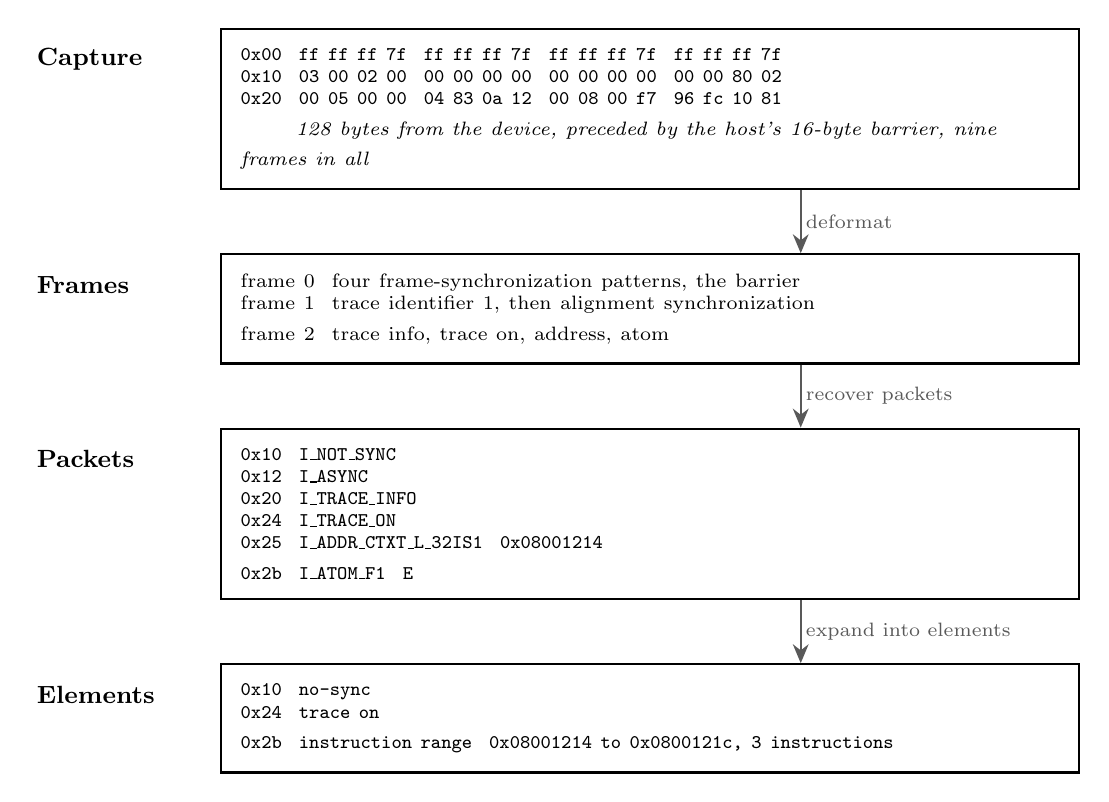
\begin{tikzpicture}[fig,
  row/.style={anchor=north west,font=\scriptsize,inner xsep=0pt,inner ysep=1pt},
  band/.style={draw,thick,anchor=north west,inner sep=2.5mm,align=left},
  dn/.style={-{Stealth[length=2.4mm,width=2mm]},thick,figdark}]

\def\W{104mm}

\node[band,text width=\W] (b1) at (0,0)
  {\ttfamily\scriptsize
   0x00\ \ ff ff ff 7f\ \ ff ff ff 7f\ \ ff ff ff 7f\ \ ff ff ff 7f\\
   0x10\ \ 03 00 02 00\ \ 00 00 00 00\ \ 00 00 00 00\ \ 00 00 80 02\\
   0x20\ \ 00 05 00 00\ \ 04 83 0a 12\ \ 00 08 00 f7\ \ 96 fc 10 81\\
   \hspace{7mm}\rmfamily\itshape 128 bytes from the device, preceded by the host's 16-byte barrier, nine frames in all};
\node[anchor=east] at ($(b1.north west)+(-2mm,-4mm)$) {\bandlbl{Capture}};

\node[band,below=8mm of b1.south west,anchor=north west,text width=\W] (b2)
  {\scriptsize
   frame 0\ \ four frame-synchronization patterns, the barrier\\
   frame 1\ \ trace identifier 1, then alignment synchronization\\
   frame 2\ \ trace info, trace on, address, atom};
\node[anchor=east] at ($(b2.north west)+(-2mm,-4mm)$) {\bandlbl{Frames}};

\node[band,below=8mm of b2.south west,anchor=north west,text width=\W] (b3)
  {\ttfamily\scriptsize
   0x10\ \ I\_NOT\_SYNC\\
   0x12\ \ I\_ASYNC\\
   0x20\ \ I\_TRACE\_INFO\\
   0x24\ \ I\_TRACE\_ON\\
   0x25\ \ I\_ADDR\_CTXT\_L\_32IS1\ \ 0x08001214\\
   0x2b\ \ I\_ATOM\_F1\ \ E};
\node[anchor=east] at ($(b3.north west)+(-2mm,-4mm)$) {\bandlbl{Packets}};

\node[band,below=8mm of b3.south west,anchor=north west,text width=\W] (b4)
  {\ttfamily\scriptsize
   0x10\ \ no-sync\\
   0x24\ \ trace on\\
   0x2b\ \ instruction range\ \ 0x08001214 to 0x0800121c,\ 3 instructions};
\node[anchor=east] at ($(b4.north west)+(-2mm,-4mm)$) {\bandlbl{Elements}};

\draw[dn] ($(b1.south)!0.35!(b1.south east)$) -- ($(b2.north)!0.35!(b2.north east)$)
      node[lbl,midway,right]{deformat};
\draw[dn] ($(b2.south)!0.35!(b2.south east)$) -- ($(b3.north)!0.35!(b3.north east)$)
      node[lbl,midway,right]{recover packets};
\draw[dn] ($(b3.south)!0.35!(b3.south east)$) -- ($(b4.north)!0.35!(b4.north east)$)
      node[lbl,midway,right]{expand into elements};

\end{tikzpicture}
\end{document}
